\documentclass[12pt]{article}


\usepackage{amssymb}
\usepackage{amsmath}
\usepackage{fullpage}
\usepackage{epsfig}
\usepackage{epstopdf}
\everymath{\displaystyle}



\begin{document}

\begin{center}
\underline{\LARGE{Chapter 3.5 Practice Problems}}
\end{center}

\noindent EXPECTED SKILLS:

\begin{itemize}

\item Be able to compute the local linear approximation of a function at a specific value. 

\item Know how to use the local linear approximation to estimate a given quantity.

\end{itemize}

\noindent PRACTICE PROBLEMS:

\medskip

\noindent {\bf For problems 1-4, calculate the Local Linear Approximation, $L(x)$, for the given function at the specified value of $x_0$.  Also, sketch $f(x)$ and $L(x)$ over the indicated interval}

\begin{enumerate}

\item $f(x)=x^2+1$, $x_0=1$, $[0,2]$

\includegraphics[scale=0.5]{start.pdf}
{{\begin{tabular}{l}
$L(x)=2x$\\
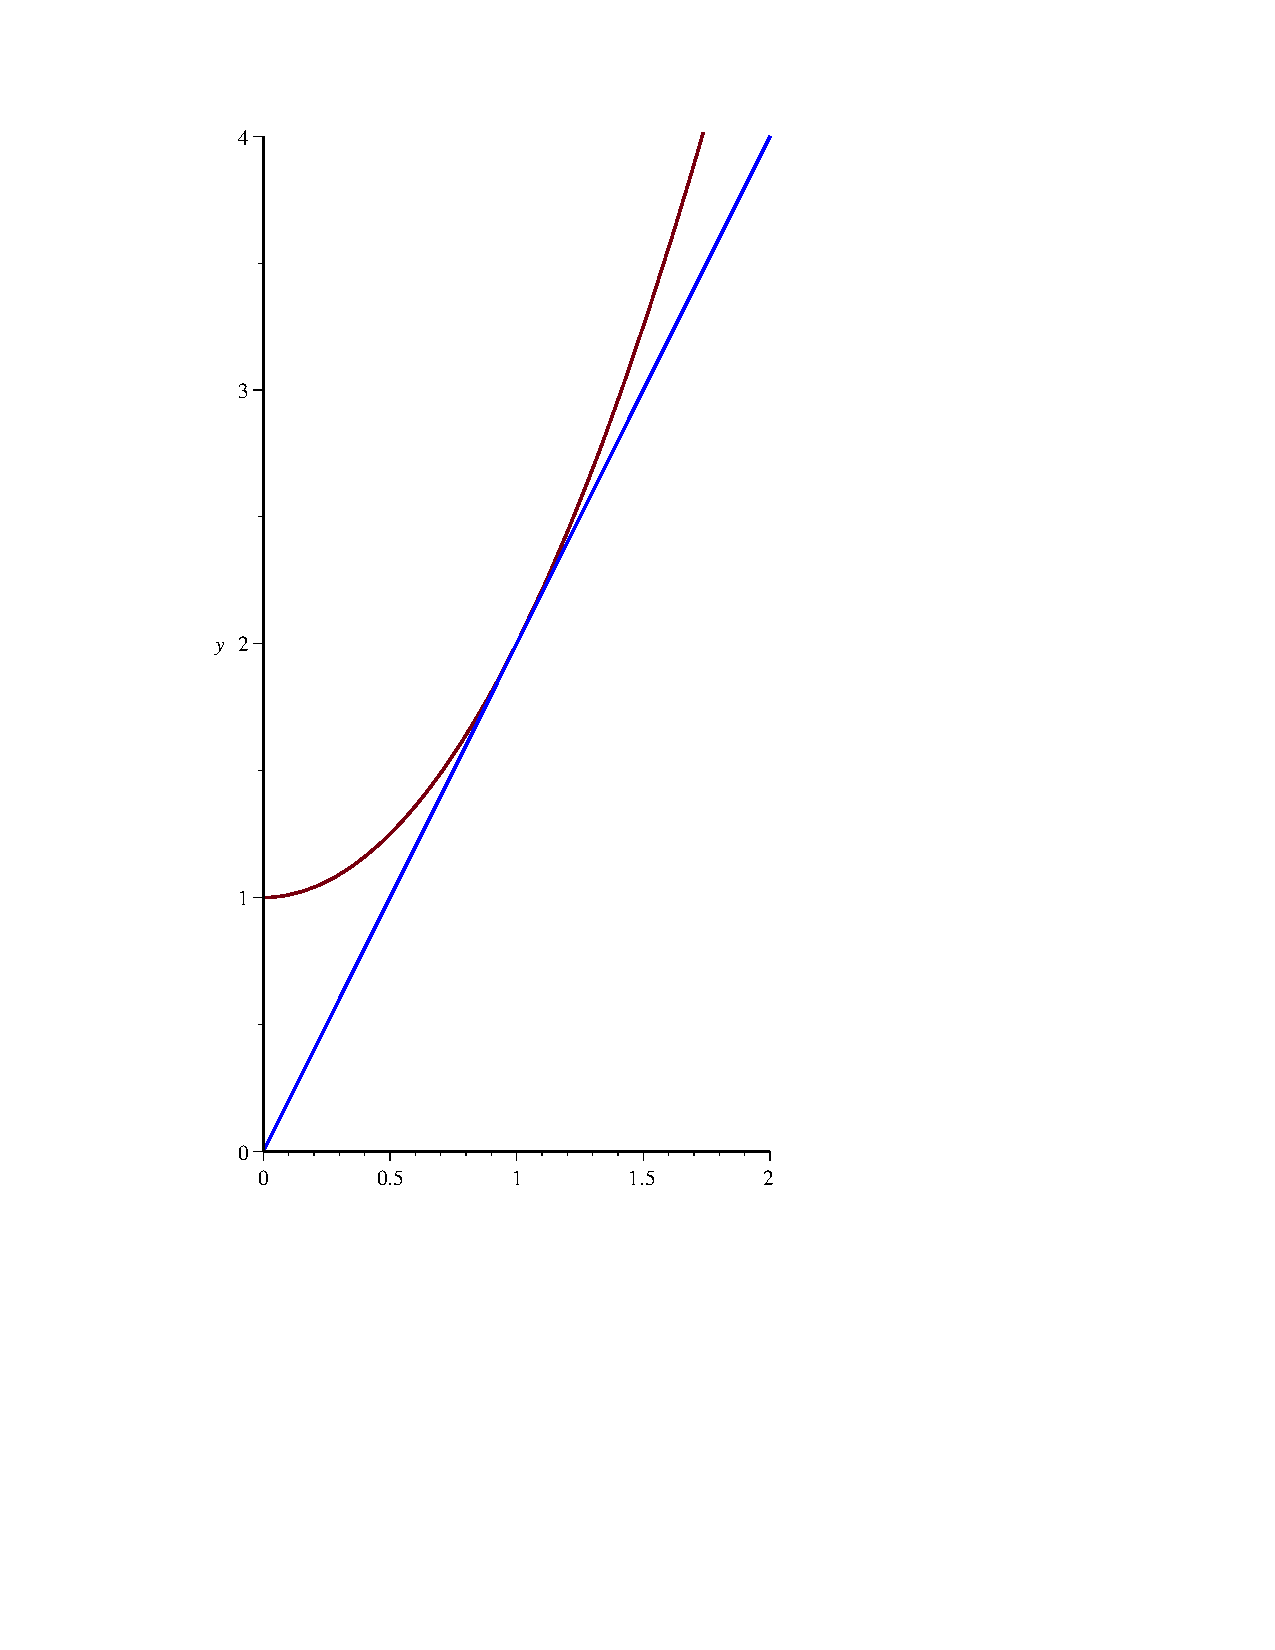
\includegraphics[scale=0.3]{graph1.pdf}
\end{tabular}
}}
\includegraphics[scale=0.5]{end.pdf}


\item $f(x)=\frac{1}{2x-1}$, $x_0=1$, $[0,2]$

\includegraphics[scale=0.5]{start.pdf}
{{\begin{tabular}{l}
$L(x)=-2x+3$\\
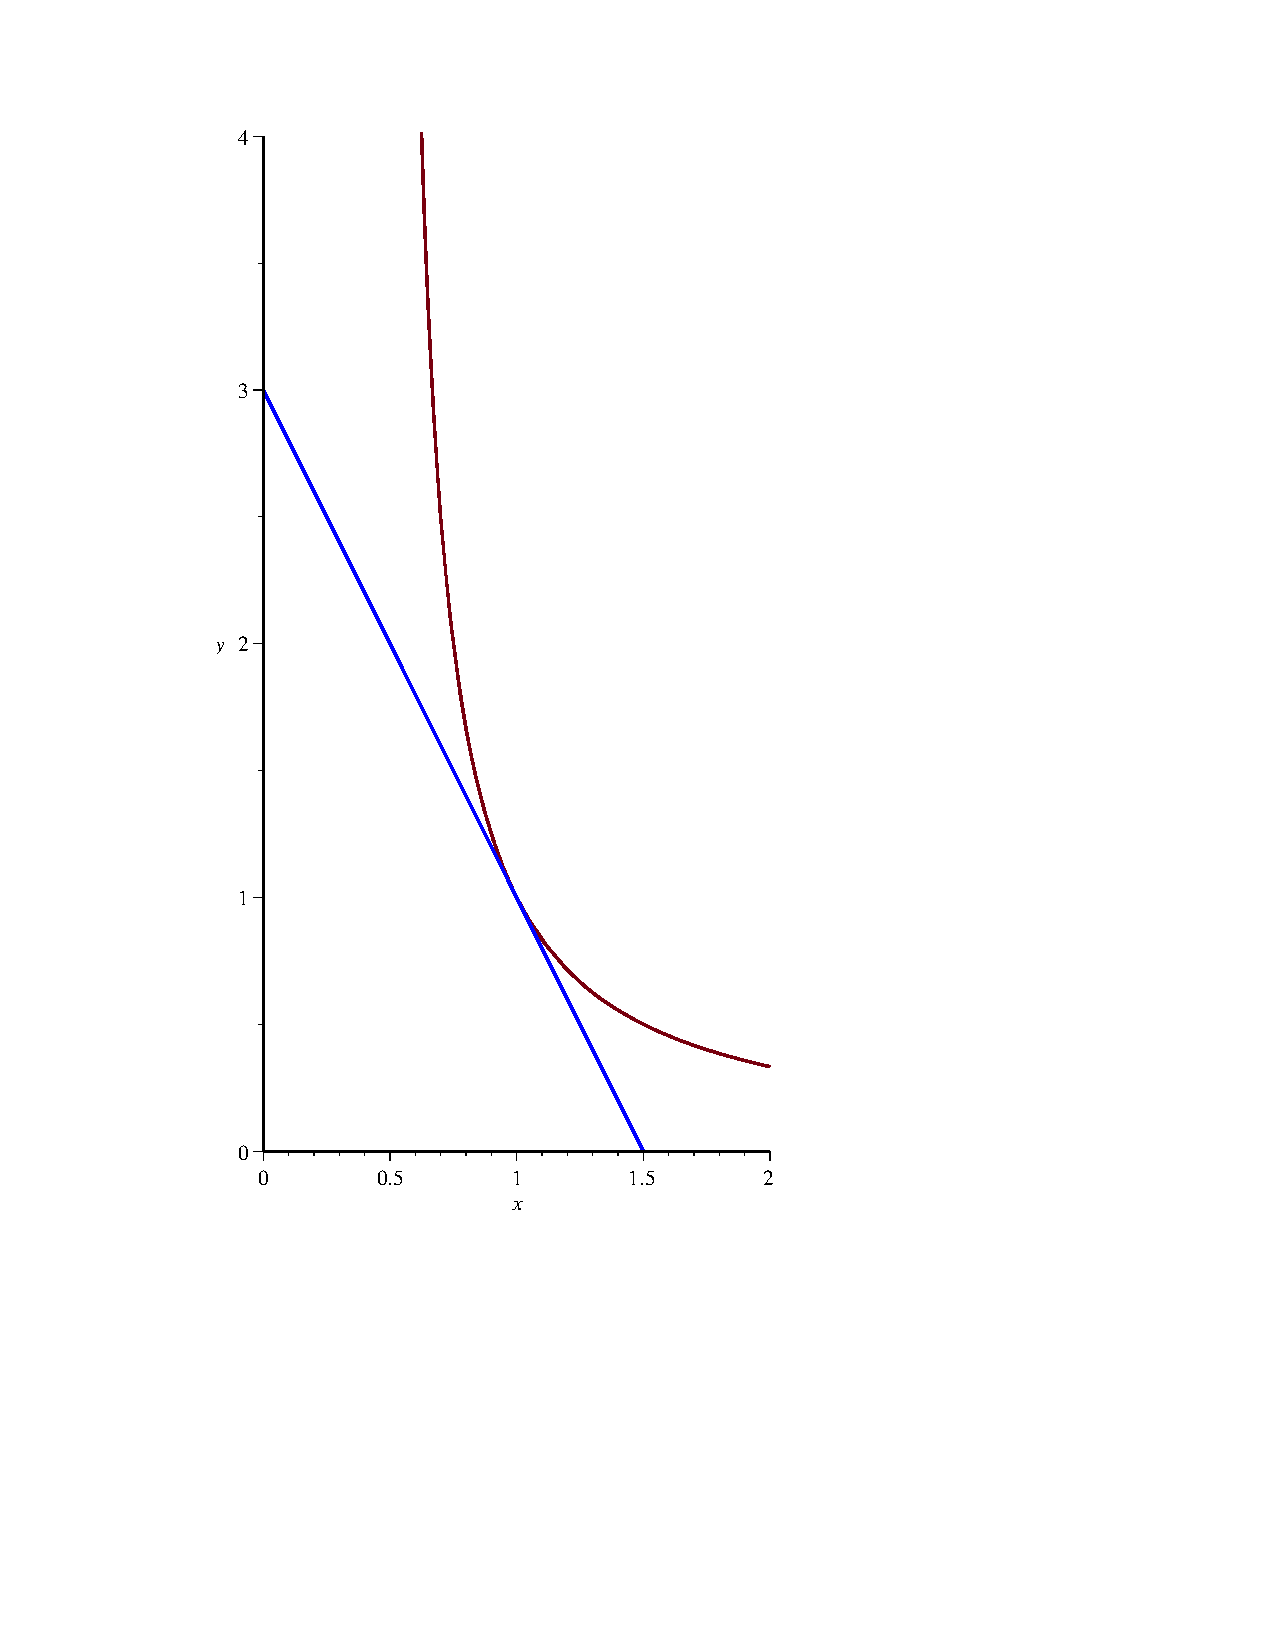
\includegraphics[scale=0.3]{graph2.pdf}
\end{tabular}
}}
\includegraphics[scale=0.5]{end.pdf}


\item $f(x)=e^{-x}$, $x_0=0$, $[-1,1]$

\includegraphics[scale=0.5]{start.pdf}
{{
\begin{tabular}{l}
$L(x)=-x+1$\\
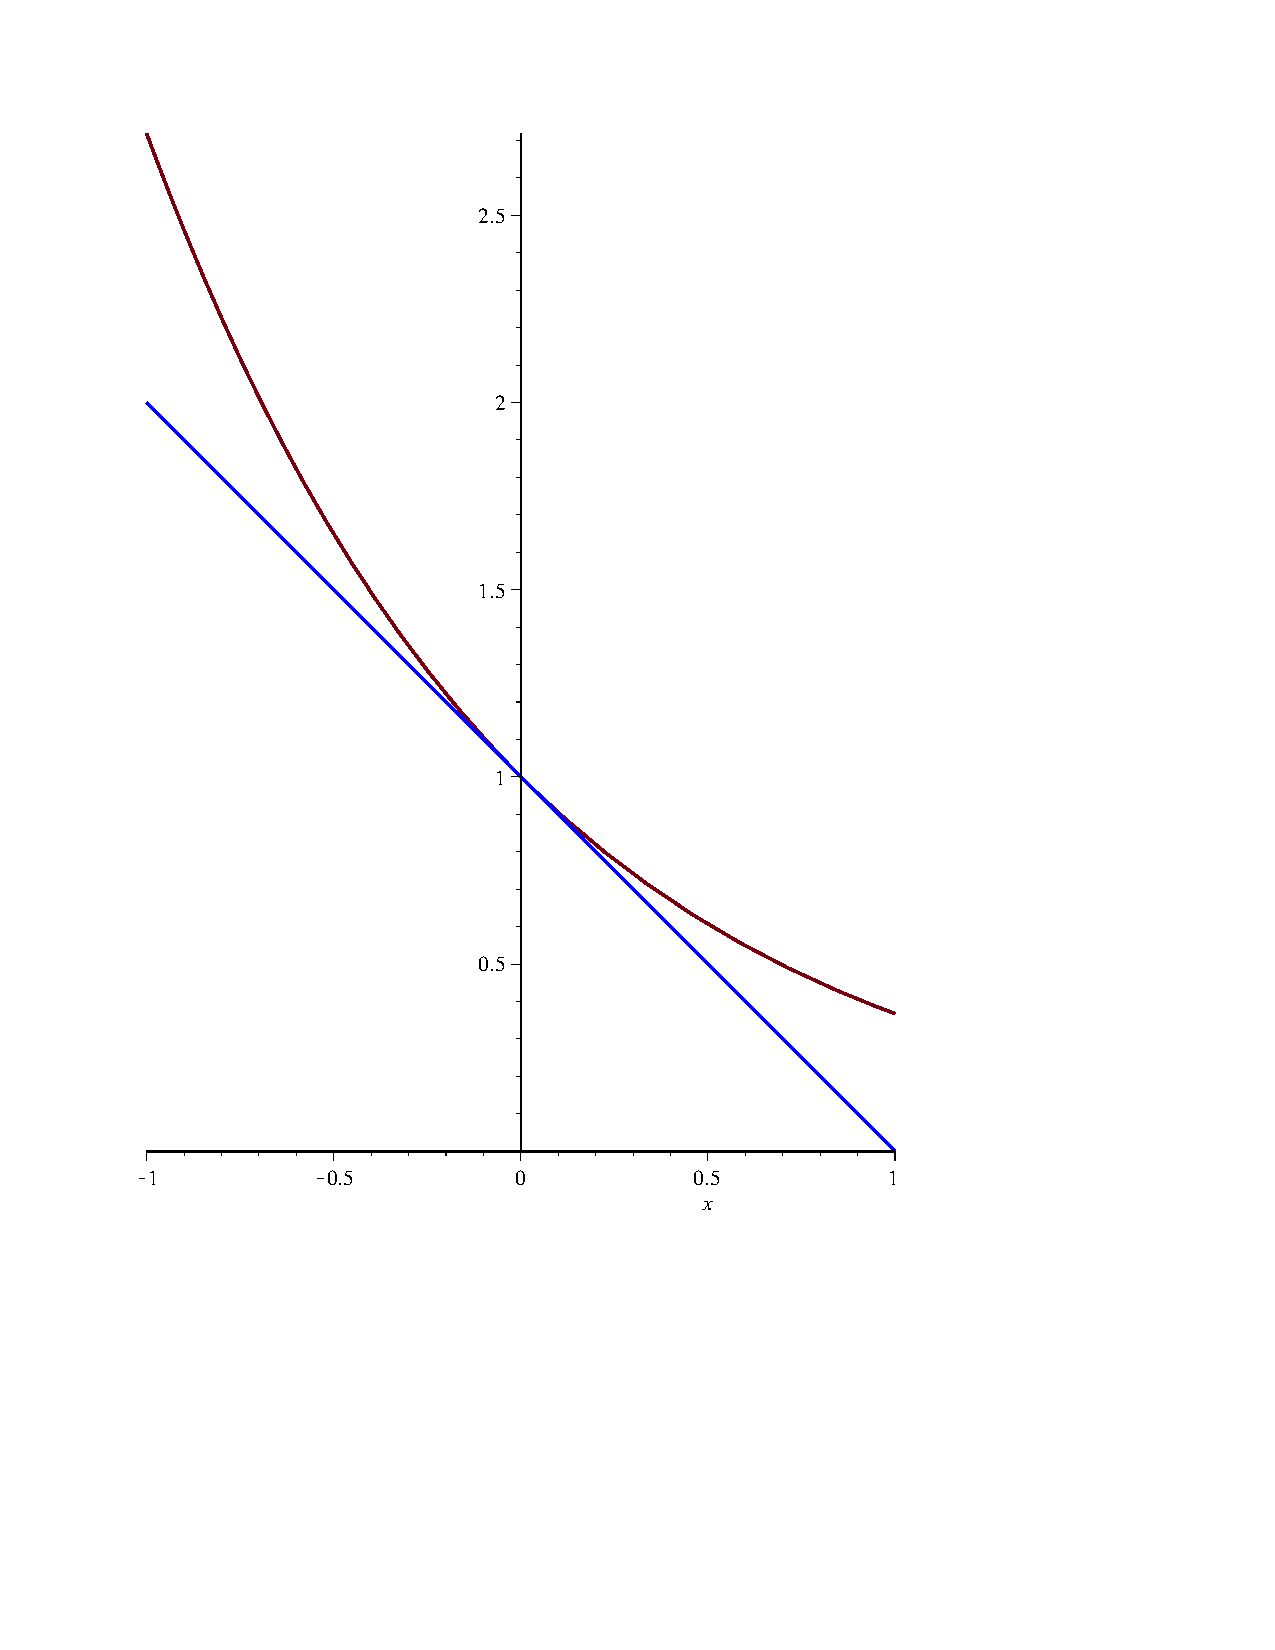
\includegraphics[scale=0.3]{graph3.pdf}
\end{tabular}
}}
\includegraphics[scale=0.5]{end.pdf}


\item $f(x) =\tan(x)$, $x_0=\frac{\pi}{4}$, $\left[0,\frac{\pi}{2}\right]$ 

\includegraphics[scale=0.5]{start.pdf}
{{\begin{tabular}{l}
$L(x)=2x-\frac{\pi}{2}+1$\\
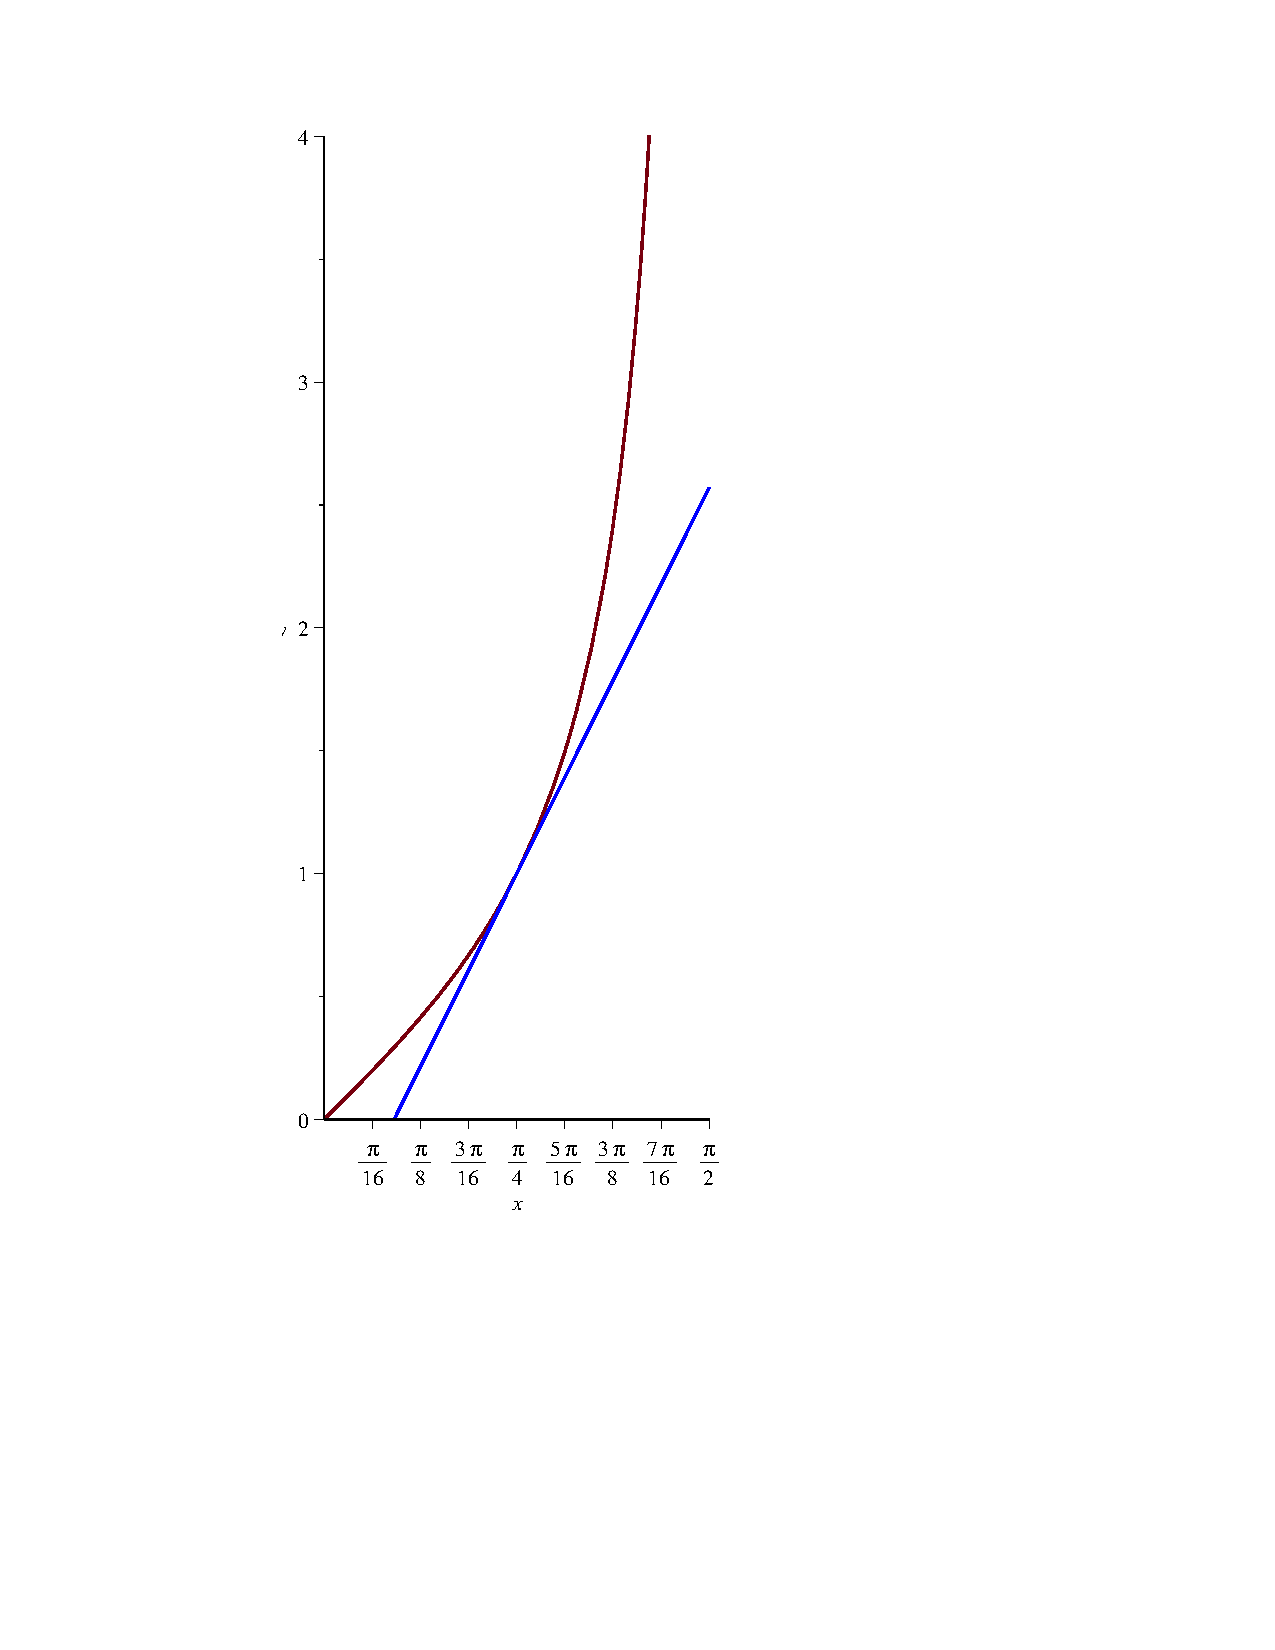
\includegraphics[scale=0.3]{graph4.pdf}
\end{tabular}
}}
\includegraphics[scale=0.5]{end.pdf}


\end{enumerate}

\noindent {\bf For problems 5-10, use an appropriate local linear approximation to approximate the following values.}

\begin{enumerate}
\setcounter{enumi}{4}

\item $(5.05)^3$ 

\includegraphics[scale=0.5]{start.pdf}
{{128.75}}
\includegraphics[scale=0.5]{end.pdf}


\item $\sqrt{101}$ 

\includegraphics[scale=0.5]{start.pdf}
{{$10.05$}}
\includegraphics[scale=0.5]{end.pdf}


\item $\sqrt[3]{28}$ 

\includegraphics[scale=0.5]{start.pdf}
{{$\frac{82}{27}$}}
\includegraphics[scale=0.5]{end.pdf}


\item $e^{0.9}$ 

\includegraphics[scale=0.5]{start.pdf}
{{$\frac{9}{10}e$}}
\includegraphics[scale=0.5]{end.pdf}


\item $\cos{0.1}$

\includegraphics[scale=0.5]{start.pdf}
{{1}}
\includegraphics[scale=0.5]{end.pdf}


\item $\sin{61^{\circ}}$ 

\includegraphics[scale=0.5]{start.pdf}
{{$\frac{\sqrt{3}}{2}+\frac{\pi}{360} $}}
\includegraphics[scale=0.5]{end.pdf}


\item Show that $(1-x)^5 \approx 1-5x$ for $x$ near 0.

\item Show that $\ln{(2x)} \approx 2x-1$ for $x$ near $\frac{1}{2}$.

\item Consider $f(x)=(x+1)^{13}$.

\begin{enumerate}

\item Compute the Local Linear Approximation of $f(x)$ at $x_0=0$.

\includegraphics[scale=0.5]{start.pdf}
{{$(x+1)^{13} \approx 1+13x$ for $x$ near 0}}
\includegraphics[scale=0.5]{end.pdf}


\item Using your approximation, estimate $(0.99)^{13}$.

\includegraphics[scale=0.5]{start.pdf}
{{$0.87$}}
\includegraphics[scale=0.5]{end.pdf}


\item Using your approximation, estimate $(1.01)^{13}$

\includegraphics[scale=0.5]{start.pdf}
{{$1.13$}}
\includegraphics[scale=0.5]{end.pdf}


\end{enumerate}

\item Let $f(x)=x^2$.

\begin{enumerate}

\item Calculate the Local Linear Approximation, $L(x)$, for $f(x)$ at $x=a$.

\includegraphics[scale=0.5]{start.pdf}
{{$L(x)=2ax-a^2$}}
\includegraphics[scale=0.5]{end.pdf}


\item Does $L(x)$ overestimate or underestimate $f(x)$ near $x=a$?  Explain.

\includegraphics[scale=0.5]{start.pdf}
{{{1\linewidth}{$L(x)$ is always an underestimate of $f(x)$ for $x$ near $a$.  Graphically, this should make sense since the tangent line to $f(x)=x^2$ is always below its graph.\\
\\
To show that $L(x)$ is always an underestimate, we will show that $L(x)\leq f(x)$ for all values of $x$.  In other words, we will show that $L(x)-f(x) \leq0$ for all $x$.  So, we compute:

\begin{align*}
L(x)-f(x) &= 2ax-a^2-x^2\\
&=-(x^2-2ax+a^2)\\
&=-(x-a)^2\\
& \leq0
\end{align*}
}}}
\includegraphics[scale=0.5]{end.pdf}


\end{enumerate}

\item {\bf Multiple Choice:} Which of the following is the best local linear approximation for $f(x)=\tan(x)$ near $\displaystyle x=\frac{\pi}{4}$?

\begin{enumerate}

\item  $\displaystyle 1+\left(x-\frac{\pi}{4}\right)$

\item $\displaystyle 1+ \frac{1}{2}\left(x-\frac{\pi}{4}\right)$

\item  $\displaystyle 1+\sqrt{2}\left(x-\frac{\pi}{4}\right)$

\item  $\displaystyle 1+2\left(x-\frac{\pi}{4}\right)$

\item $\displaystyle 2+2\left(x-\frac{\pi}{4}\right)$

\end{enumerate}

\includegraphics[scale=0.5]{start.pdf}
{{D}}
\includegraphics[scale=0.5]{end.pdf}


\end{enumerate}

\end{document}